\documentclass{article}
%----------------------------------------------------------------------
\usepackage[polish]{babel}
\usepackage[utf8]{inputenc}
\usepackage[T1]{fontenc}
\usepackage[a4paper,top=2cm,bottom=2cm,left=3cm,right=3cm,marginparwidth=1.75cm]{geometry}
\usepackage{amsmath}
\usepackage{graphicx}
\usepackage[colorlinks=true, allcolors=black]{hyperref}
\usepackage{blindtext}
\usepackage{nomencl}
\usepackage{listings}
\usepackage{xcolor}
\usepackage{float}
\usepackage{etoolbox}
\usepackage{tabularx}
\usepackage{array}
\usepackage{enumitem}
\usepackage{amsfonts}
%----------------------------------------------------------------------
\begin{document}

\begin{titlepage}
    \centering
    \vspace{1.5cm}
    
\includegraphics[width=0.9\textwidth]{university-logo.png} \\
    \vspace{2.5cm}
    {\fontsize{30}{20}\selectfont \textbf{Metody Sztucznej Inteligencji 2} \par}
    \vspace{1.5cm}
    {\fontsize{25}{20}\selectfont Zastosowanie Monte-Carlo Tree Search do implementacji sztucznej inteligencji w grze Breakthrough\par}
    \vspace{1.5cm}
    {\fontsize{18}{20}\selectfont Konspekt\par}
    \vspace{1.5cm}
    {\fontsize{12}{20}\selectfont Zespół: \\ inż. Adam Grącikowski \\ inż. Piotr Iśtok \par}
    \vspace{0.5cm}
    {\fontsize{12}{20}\selectfont Prowadzący: \\ mgr inż. Bartłomiej Olechno \\ prof. dr hab. inż. Jacek Mańdziuk \par}
    
    \vfill
    Oświadczamy, że niniejsza praca, stanowiąca podstawę do uznania osiągnięcia efektów uczenia się z przedmiotu \textit{Metody Sztucznej Inteligencji 2}, została wykonana samodzielnie. 

    \vspace{1cm}
    
    Warszawa, \today
    
\end{titlepage}

%----------------------------------------------------------------------
\tableofcontents
\newpage

%----------------------------------------------------------------------

\section{Wprowadzenie}

\subsection{Cel projektu}

Celem projektu jest zaprojektowanie, implementacja oraz ewaluacja agenta sztucznej inteligencji zdolnego do prowadzenia rozgrywki w dwuosobową grę o sumie zerowej z pełną informacją – ,,Breakthrough'' – z wykorzystaniem algorytmu Monte-Carlo Tree Search (MCTS)~\cite{coulom2006efficient}, ze szczególnym uwzględnieniem wariantu Upper Confidence Bound Applied to Trees (UCT)~\cite{kocsis2006bandit}.

W ramach projektu przeprowadzona zostanie weryfikacja i porównanie skuteczności działania standardowej wersji algorytmu UCT w zestawieniu z jego rozszerzeniami, autorskimi podejściami heurystycznymi dedykowanymi wybranej grze, a także w bezpośredniej konfrontacji z ludzkimi graczami. Projekt ma na celu wykazanie wpływu modyfikacji parametrów algorytmicznych oraz reguł samej gry na wydajność i jakość podejmowanych przez agenta decyzji.

\subsection{Zakres projektu}

Zakres prac w ramach projektu obejmuje fazę implementacyjną, badawczą oraz analityczną, które składają się na następujące zadania:

\begin{itemize}
    \item Implementacja środowiska gry: Stworzenie w pełni funkcjonalnego środowiska dla gry ,,Breakthrough''. Środowisko będzie architektonicznie dostosowane do przeprowadzania eksperymentów poprzez parametryzację zasad gry.
    \item Implementacja algorytmów sztucznej inteligencji: agenta bazowego, jego dwóch wariantów usprawniających, a także agenta eksperckiego.
    \item Weryfikacja hipotez badawczych: Sformułowanie i weryfikacja (przy pomocy zautomatyzowanych testów -- rozgrywek pomiędzy agentami) postawionych hipotez.
    \item Moduł interakcji z człowiekiem: Zbudowanie interfejsu graficznego, który umożliwi rozgrywkę człowieka z wybranym agentem.
    \item Ewaluacja z udziałem ludzi: Zrealizowanie rozgrywek pomiędzy zaimplementowanymi agentami a grupą badawczą, składającą się z minimum 5 osób.
    \item Analiza i raportowanie: Zestawienie zebranych danych ilościowych i jakościowych, analiza statystyczna wyników przeprowadzonych turniejów oraz weryfikacja postawionych hipotez badawczych w raporcie końcowym.
\end{itemize}

\newpage

\section{Gra ,,Breakthrough'' jako środowisko badawcze}

\subsection{Zasady gry} 

Gra ,,Breakthrough'' to deterministyczna, dwuosobowa gra planszowa należąca do kategorii gier abstrakcyjnych. W klasycznym wariancie jest rozgrywana na planszy o wymiarach $8 \times 8$ pól, chociaż mechanika gry w naturalny sposób skaluje się do przestrzeni o innych wymiarach ($N \times M$). 

Każdy z graczy rozpoczyna rozgrywkę z zestawem pionów (16 figur na gracza w wariancie $8 \times 8$), które w początkowym ułożeniu zajmują dwa skrajne rzędy planszy po stronach obu przeciwników. Ruch polega na przemieszczeniu własnego piona o dokładnie jedno pole do przodu – w kierunku prostopadłym lub po skosie (Rysunek \ref{fig:board_example}). 

Bicie figur przeciwnika uwarunkowane jest regułą znaną z tradycyjnych szachów –- odbywa się wyłącznie na polach leżących po skosie z przodu przemieszczanej figury. Pion przeciwnika po zbiciu jest trwale usuwany z przestrzeni gry. Nie istnieje możliwość poruszania się ani bicia do tyłu czy w poziomie. Rozgrywka kończy się w momencie spełnienia jednego z dwóch warunków zwycięstwa:

\begin{enumerate}
    \item Pion jednego z graczy dotrze do przeciwległego końca planszy (ostatniego rzędu startowego przeciwnika) – co stanowi tytułowe przebicie (ang. \textit{breakthrough}).
    \item Gracz straci wszystkie swoje figury w wyniku bić, przez co nie dysponuje żadnym legalnym ruchem.
\end{enumerate}

\begin{figure}[h]
    \centering
    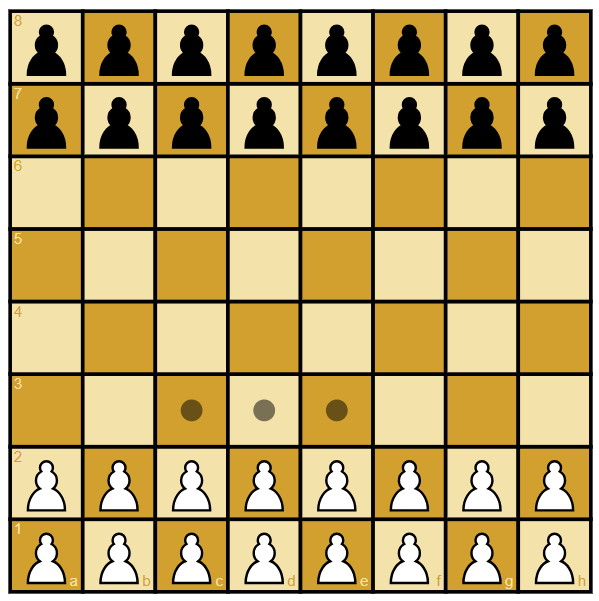
\includegraphics[width=0.5\textwidth]{images/board_example.png}
    \caption{Stan początkowy planszy dla gry ,,Breakthrough''. Szare kropki oznaczają pola, na których może się znaleźć pion na pozycji \texttt{d2} w wyniku pojedynczego półruchu (ang. \textit{ply}).}
    \label{fig:board_example}
\end{figure}

\subsection{Właściwości i złożoność obliczeniowa}

,,Breakthrough'' jest grą o sumie zerowej, charakteryzującą się pełną (doskonałą) informacją oraz całkowitym brakiem elementu losowego. Złożoność obliczeniowa gry rośnie wykładniczo wraz ze wzrostem rozmiaru planszy.

Zgodnie z analizą przeprowadzoną przez Saffidine, Jouandeau i Cazenave'a \cite{saffidine2012solving}, górne ograniczenie przestrzeni stanów (ang. \textit{state-space complexity}) dla planszy o wymiarach $N \times M$ wyraża się wzorem \ref{eq:state_space_complexity}. 

\begin{equation}
    2^{2N} \times 3^{(M-2)N}
    \label{eq:state_space_complexity}
\end{equation}

\noindent
Zależność ta wynika z faktu, że skrajne rzędy mogą zawierać wyłącznie piony jednego koloru lub puste pola, podczas gdy na pozostałych rzędach mogą znajdować się figury obu graczy. Z kolei średni współczynnik rozgałęzienia (ang. \textit{branching factor}) dla tego wariantu szacowany jest na około od 20 do 30 możliwych ruchów na turę \cite{saffidine2012solving}. 

Z uwagi na sposób poruszania się pionów (wyłącznie do przodu), w grafie stanów gry nie występują cykle, a maksymalna długość rozgrywki jest ściśle i deterministycznie ograniczona. Powyższe właściwości sprawiają, że ,,Breakthrough'' stanowi odpowiednie środowisko testowe dla algorytmów przeszukiwania drzewa, takich jak Monte-Carlo Tree Search.

\subsection{Reprezentacja stanu gry} 

Stan planszy zostanie zamodelowany z wykorzystaniem tzw. tablic bitowych (ang. \textit{bitboards}). Pełny obraz układu figur na planszy reprezentowany będzie przy pomocy dwóch całkowitoliczbowych zmiennych bez znaku o rozmiarze 128 bitów (typ \texttt{u128}). Pierwsza ze zmiennych będzie kodować pozycje białych pionów (bit o wartości 1 na $i$-tym miejscu oznacza obecność piona na $i$-tym polu, a 0 jego brak), natomiast druga zmienna analogicznie będzie przechowywać pozycje pionów czarnych.

Stan planszy uzupełni informacji o tym, który z graczy dysponuje aktualnie prawem ruchu. W implementacji wykorzystana zostanie zmienna logiczna lub typ wyliczeniowy (1 bajt). Ponieważ gra nie zawiera mechanik takich jak roszady czy bicia w przelocie, nie ma konieczności przechowywania historii ruchów ani dodatkowych flag stanu. 

Całkowity rozmiar tak zdefiniowanej struktury wynosi 33 bajty (32 bajty na obie tablice \texttt{u128} oraz 1 bajt na identyfikator gracza).

\subsubsection{Operacje bitowe}

Zmiana stanu planszy i wyznaczanie wszystkich legalnych ruchów zostanie zrealizowana za pomocą podstawowych operacji bitowych. Zaletą takiej reprezentacji efektywność operacji masowych i niewielki rozmiar.

\subsubsection{Ograniczenia reprezentacji}

Typ \texttt{u128} determinuje fizyczny limit obsługiwanej przestrzeni –- pozwala na mapowanie najwyżej 128 pól. Zastosowana implementacja umożliwia więc eksperymentowanie na planszach o maksymalnym wymiarze $11 \times 11$ (121 pól).

Główne eksperymenty badawcze planowane są dla wariantów planszy o rozmiarach mniejszych niż klasyczne $8 \times 8$. Zabieg ten ma na celu redukcję złożoności przestrzeni stanów i umożliwienie algorytmom przeszukiwania osiągnięcie większej głębokości w akceptowalnym czasie obliczeniowym. 

W procesie selekcji środowisk testowych konieczne jest pominięcie wariantów, które zostały już w literaturze silnie rozwiązane. Zgodnie z dotychczasowymi dowodami~\cite{saffidine2012solving}, z puli testowej wykluczone zostaną następujące konfiguracje:

\begin{itemize}
    \item $6 \times 6$ (wygrywa pierwszy gracz),
    \item $6 \times 5$ (wygrywa drugi gracz),
    \item $5 \times 5$ (wygrywa drugi gracz),
    \item $3 \times 7$ (wygrywa drugi gracz).
\end{itemize}

\newpage

\section{Algorytmy}

\subsection{Klasyczny algorytm Monte-Carlo Tree Search (UCT)}

Algorytm Monte-Carlo Tree Search (MCTS) w wariancie UCT (ang. \textit{Upper Confidence Bound Applied to Trees}) to probabilistyczna i heurystyczna metoda przeszukiwania przestrzeni stanów. Algorytm ten buduje drzewo gry w sposób asymetryczny, alokując najwięcej zasobów obliczeniowych na ewaluację najbardziej obiecujących wariantów.

Każdy węzeł w drzewie gry ,,Breakthrough'' przechowuje stan planszy (reprezentowany przez tablice bitowe), informacje o graczu wykonującym ruch oraz statystyki odwiedzin i zwycięstw.

Proces decyzyjny algorytmu opiera się na ciągłym powtarzaniu cyklu operacji. Pojedyncza iteracja algorytmu składa się z sekwencyjnego wykonania dokładnie czterech faz: selekcji, ekspansji, symulacji oraz propagacji wstecznej. Ten pełny cykl jest powtarzany wielokrotnie, aż do wyczerpania zadanego budżetu obliczeniowego (np. ustalonego limitu czasu lub maksymalnej liczby iteracji).

\subsubsection{Selekcja}

Pojedyncza iteracja rozpoczyna się od węzła głównego (korzenia reprezentującego aktualny stan gry na planszy). Algorytm iteracyjnie schodzi w dół drzewa, wybierając w każdym kroku optymalny węzeł potomny. Faza ta trwa tak długo, jak długo rozpatrywany węzeł jest w pełni rozwinięty (ang. \textit{fully expanded}) –- oznacza to, że dla wszystkich możliwych do wykonania z tego stanu legalnych ruchów, dodano już do drzewa odpowiadające im węzły potomne.

Wybór optymalnej ścieżki na etapach w pełni wyekspandowanych realizowany jest za pomocą formuły UCB1, która rozwiązuje dylemat pomiędzy eksploatacją znanych, dobrych zagrań, a eksploracją rzadziej odwiedzanych gałęzi. Formułę tę można przedstawić za pomocą następującego wyrażenia~\cite{kocsis2006bandit}:

$$\frac{w_i}{n_i} + C \sqrt{\frac{\ln N}{n_i}}$$

\noindent
gdzie:

\begin{itemize}
    \item $w_i$ to łączna liczba symulacji zakończonych zwycięstwem, przeprowadzonych przez dany węzeł potomny $i$,
    \item $n_i$ to łączna liczba wszystkich odwiedzin rozpatrywanego węzła potomnego $i$,
    \item $N$ to całkowita liczba odwiedzin węzła-rodzica,
    \item $c$ to stała eksploracji (w literaturze często przyjmuje się $c = \sqrt{2}$).
\end{itemize}

\noindent
Pierwszy składnik sumy odpowiada za eksploatację -- jego duża wartość oznacza, że dana ścieżka ma wysoki współczynnik zwycięstw. Drugi składnik sumy odpowiada za eksplorację -- jego wartość rośnie, gdy węzeł potomny był rzadko odwiedzany w stosunku do całkowitej liczby wizyt w jego węźle-rodzicu.

\subsubsection{Ekspansja}

Kiedy faza selekcji natrafi na węzeł, który nie jest w pełni rozwinięty (brakuje w nim reprezentacji przynajmniej jednego legalnego ruchu), cykl przechodzi do fazy ekspansji. Z wykorzystaniem operacji na tablicach bitowych (\texttt{u128}) generowany jest zbiór wszystkich dopuszczalnych w danym stanie zagrań. Następnie algorytm wybiera (najczęściej losowo) jeden z dotychczas niezbadanych ruchów. Powstały w ten sposób nowy układ pionów jest dodawany do drzewa jako nowy węzeł liścia. Jego początkowe statystyki inicjalizowane są wartościami zerowymi ($w_i = 0$, $n_i = 0$).

\subsubsection{Symulacja}

Począwszy od nowo utworzonego węzła liścia, algorytm przeprowadza symulację rozgrywki (ang. \textit{rollout}) aż do osiągnięcia stanu końcowego. W klasycznym UCT symulacja ta polega na wybieraniu całkowicie pseudolosowych, dopuszczalnych ruchów przez obu graczy. Z uwagi na wyścigowy charakter gry ,,Breakthrough'' oraz brak możliwości poruszania się pionów do tyłu, faza ta wykonuje się w sposób wysoce zoptymalizowany i zawsze zbiega do jednoznacznego wyniku (przebicia się na drugą stronę planszy lub utraty wszystkich figur).

\subsubsection{Propagacja wsteczna}

Po zakończeniu symulacji, determinowany jest jej ostateczny wynik (zwycięstwo białych lub czarnych). Algorytm przemieszcza się od nowo utworzonego liścia w górę drzewa, z powrotem do korzenia, aktualizując statystyki w każdym odwiedzonym węźle. Licznik wizyt ($n_i$) inkrementowany jest o 1, a do licznika zwycięstw ($w_i$) dodawana jest nagroda zależna od perspektywy gracza w danym węźle (np. 1 w przypadku wygranej symulacji, 0 w przypadku przegranej).

\subsubsection{Wybór ostatecznego ruchu}

Po wyczerpaniu dostępnego budżetu obliczeniowego, pętla iteracyjna zostaje przerwana. Na tym etapie algorytm podejmuje ostateczną decyzję o wyborze ruchu, analizując wyłącznie dzieci węzła głównego (korzenia). Zgodnie z polityką odpornego dziecka (ang. \textit{robust child})~\cite{browne2012survey}, w asymetrycznym drzewie optymalnym ruchem jest ten, który algorytm zdecydował się odwiedzić najwięcej razy w trakcie wszystkich iteracji. Ostateczny ruch $a^*$ wybierany jest zgodnie z poniższym wzorem:

$$a^* = \arg\max_{a \in \mathcal{A}(s_0)} n_a$$

\noindent
gdzie:

\begin{itemize}
    \item $a^*$ to optymalny ruch (akcja) zwrócony przez algorytm,
    \item $\mathcal{A}(s_0)$ to zbiór wszystkich legalnych ruchów dostępnych w bieżącym stanie gry (korzeniu $s_0$),
    \item $n_a$ to całkowita liczba odwiedzin węzła potomnego, do którego prowadzi wykonanie akcji $a$.
\end{itemize}

\subsubsection{Budżet obliczeniowy i warunki zakończenia}

Algorytm MCTS należy do rodziny algorytmów typu \textit{anytime}, co oznacza, że jego działanie może zostać przerwane w dowolnej iteracji, a drzewo przeszukiwań wciąż będzie w stanie zwrócić najlepszy znaleziony do tej pory ruch.

Zaimplementowane i wykorzystane będą dwa niezależne warunki zakończenia przeszukiwania, dobierane w zależności od specyfiki przeprowadzanego eksperymentu:

\begin{enumerate}
    \item Limit iteracji: Wykorzystywany podczas zautomatyzowanych turniejów (ang. \textit{self-play}) w fazie weryfikacji hipotez badawczych.
    \item Limit czasu: Wykorzystywany podczas interakcji algorytmu z człowiekiem.
\end{enumerate}

\subsection{Proponowane modyfikacje UCT}
\subsubsection{Pierwsza modyfikacja: Heurystyka AMAF i algorytm RAVE}

Głównym ograniczeniem klasycznego wariantu UCT jest wolne tempo aktualizacji statystyk dla nowo odwiedzonych węzłów. W standardowym podejściu, wynik z fazy symulacji służy do aktualizacji wyłącznie tych węzłów, które leżą dokładnie na wybranej ścieżce od korzenia do liścia. 

W celu przyspieszenia zbieżności algorytmu na wczesnych etapach przeszukiwania, zaimplementowana zostanie modyfikacja oparta na heurystyce AMAF (ang. \textit{All-Moves-As-First}) oraz algorytmie RAVE (ang. \textit{Rapid Action Value Estimation}), zaproponowanym przez Sylvaina Gelly'ego oraz Davida Silvera \cite{gelly2007monte}. Heurystyka AMAF zakłada, że jakość danego ruchu jest w dużej mierze niezależna od momentu, w którym jest on wykonywany. Jeśli przykładowy ruch $a$ wykonany został na dowolnym etapie symulacji (nawet głęboko w fazie losowego \textit{rolloutu}) i doprowadził do zwycięstwa, heurystyka ta traktuje to jako dowód, że ruch ten byłby prawdopodobnie równie skuteczny, gdyby został wykonany jako pierwszy.

Największa zmiana względem klasycznej wersji zachodzi w fazie propagacji. Podczas tego etapu, algorytm RAVE będzie aktualizował dwa niezależne zestawy statystyk każdego odwiedzanego węzła potomnego $i$:
\begin{enumerate}
    \item Statystyki standardowe: Licznik odwiedzin $n_i$ oraz licznik zwycięstw $w_i$ (analogiczne do podstawowej wersji).
    \item Statystyki heurystyki: Licznik odwiedzin AMAF $\tilde{n}_i$ oraz licznik zwycięstw AMAF $\tilde{w}_i$. Mechanizm ich aktualizacji odrzuca warunek ścisłej sekwencyjności. Niech węzeł potomny $i$ reprezentuje stan gry powstały w wyniku wykonania akcji $a$ w jego węźle-rodzicu. Podczas propagacji wstecznej algorytm weryfikuje, czy akcja $a$ należy do zbioru wszystkich posunięć zrealizowanych przez odpowiadającego jej gracza w trakcie trwania całej bieżącej iteracji (zarówno w fazie selekcji, jak i losowej symulacji). Jeśli weryfikacja przebiegnie pomyślnie, liczniki $\tilde{n}_i$ oraz $\tilde{w}_i$ są odpowiednio inkrementowane. Dzięki temu aktualizacja następuje niezależnie od tego, na jakiej głębokości i w jakiej kolejności ruch $a$ faktycznie wystąpił w rozpatrywanej partii.
\end{enumerate}

Zmodyfikowana jest również faza selekcji. Podczas jej, algorytm wykorzystuje wartość eksploatacji węzła, określoną jako ważona średnią liniową wartości klasycznej $V_{MCTS}$ oraz wartości heurystycznej $V_{AMAF}$ \cite{gelly2007monte}:

$$V_{RAVE} = (1 - \beta) \frac{w_i}{n_i} + \beta \frac{\tilde{w}_i}{\tilde{n}_i}$$

\noindent
Parametr $\beta$ określa stopień ufności algorytmu wobec heurystyki AMAF i jest definiowany zgodnie z poniższym wzorem:

$$\beta = \frac{k}{k + n_i}$$

\noindent
gdzie $k$ jest hiperparametrem, określającym po ilu klasycznych odwiedzinach węzła ($n_i = k$), wagi obu estymatorów zrównają się ($\beta = 0.5$). Najczęściej jego wartość ustawiana jest w przedziale $[200;700]$. Dzięki temu, że wraz ze wzrostem całkowitej liczby wizyt $n_i$, wartość $\beta$ asymptotycznie dąży do zera, algorytm płynnie przechodzi od szybkiej, ale zaszumionej eksploracji AMAF, do precyzyjnej, klasycznej ewaluacji UCT. Obliczona wartość $V_{RAVE}$ zastępuje pierwszy składnik w standardowej formule UCB1.

\subsubsection{Druga modyfikacja: Usprawniona faza symulacji (ang. \textit{Heavy Playouts})}

Klasyczny algorytm UCT w fazie symulacji wybiera ruchy zgodnie z jednostajnym rozkładem prawdopodobieństwa. Gra ,,Breakthrough'' charakteryzuje się dużą liczbą bić, więc całkowicie losowa faza \textit{rollout} prowadzi do generowania mało realnych scenariuszy, co zniekształca statystyki zwycięstw w węzłach. Druga zaproponowana modyfikacja polega na wprowadzeniu mechanizmu \textit{Heavy Playouts} \cite{browne2012survey}, w którym faza symulacji jest sterowana wiedzą dziedzinową.

Zamiast wyboru losowego, agent wykorzystuje funkcję oceny pozycji $E$ dla każdego możliwego ruchu agenta. Funkcja ta zostanie szczegółowo zdefiniowana w rozdziale \ref{sub:ewaluacja_stanu_gry} na potrzeby agenta heurystycznego. Dokonuje ona analizy stanu planszy pod kątem przewagi materialnej, zaawansowania pionów oraz struktur obronnych z wykorzystaniem wydajnych operacji bitowych.

Aby zapobiec determinizmowi i przewidywalności ruchów, zastosowana polityka symulacji została oparta na podejściu $\epsilon$-zachłannym (ang. $\epsilon$-greedy) \cite{sutton2018reinforcement}. Polega ona na tym, że agent w fazie \textit{rollout} będzie losował, czy wykonywać przypadkowy ruch legalny, czy najlepszy według funkcji oceny $E$ w bieżącym stanie symulacji. Wykonanie ruchu losowego jest następuje z prawdopodobieństwem $\epsilon$, gdzie przyjęto, że $\epsilon = 0,1$, a z prawdopodobieństwem $1-\epsilon$ agent kieruje się tylko i wyłącznie heurystyką.

Wprowadzenie ciężkich symulacji pozwala na generowanie ścieżek o wyższej jakości merytorycznej, co sprawia, że wyniki \textit{rolloutów} są bliższe rzeczywistej sile gry agentów. Wadą tej modyfikacji jest koszt obliczeniowy. W każdej operacji w fazie symulacji wymagane jest wygenerowania wszystkich legalnych ruchów, ich ocenienie i wybór najlepszego z nich.

\subsection{Podejście heurystyczne}

Jako punkt odniesienia (ang. \textit{baseline}) dla algorytmu MCTS i jego modyfikacji, zostanie zaimplementowany wyspecjalizowany agent heurystyczny. Podejście to składa się z dwóch elementów: statycznej funkcji oceny pozycji (wykorzystującej wiedzę dziedzinową dla gry ,,Breakthrough'') oraz deterministycznego algorytmu przeszukiwania drzewa gry.

\subsubsection{Ewaluacja stanu gry} \label{sub:ewaluacja_stanu_gry}

Funkcja oceny pozycji $E$ będzie zdefiniowana jako liniowa suma ważona czterech cech (ang. \textit{features}), wyliczanych ze stanu planszy za pomocą operacji bitowych:

\begin{itemize}
    \item Zaawansowanie pionów: Różnicę pomiędzy najbardziej wysuniętym pionem gracza a najbardziej wysuniętym pionem przeciwnika względem ich docelowych linii końcowych.
    \item Przewaga materialna: Różnica w całkowitej liczbie figur pozostających na planszy.
    \item Struktury obronne: Promowanie zwartych formacji. Agent otrzymuje premię za każdego piona, który znajduje się na polu chronionym od tyłu (po skosie) przez inną własną figurę.
    \item Kara za krawędzie: Zniechęcanie do prowadzenia figur skrajnymi kolumnami planszy (\texttt{A} oraz \texttt{H}). Piony znajdujące się na krawędziach dysponują jedynie dwiema, a nie trzema legalnymi opcjami ruchu.
\end{itemize}

\noindent
W przypadku wykrycia warunków zakończenia gry (wygrana lub przegrana), funkcja pomija powyższe obliczenia i zwraca wysoką lub niską wartość (nieskończoność), dołączając do niej premię lub karę zależną od głębokości przeszukiwania. Dzięki temu preferowane są najszybsze ścieżki do zwycięstwa i maksymalne opóźnianie ewentualnej porażki.

\subsubsection{Proces decyzyjny}

Wybór ostatecznego ruchu realizowany jest za pomocą algorytmu Minimax \cite{russell2010artificial}. Planowane jest zastosowanie przeszukiwania z ograniczoną, niewielką głębokością (np. 3 lub 4 półtury). Możliwości agenta będą przypominały możliwości ludzkie. Ludzie nie są w stanie przeliczyć drzewa gry do samego końca -- zamiast tego planują swoje akcje na kilka kroków w przód, a następnie intuicyjnie ocenia, czy powstała w ten sposób sytuacja na planszy jest dla niego korzystna. Płytki Minimax połączony z ekspercką funkcją oceny $E$ stanowi odzwierciedlenie tego procesu.

Dodatkowo, klasyczny algorytm Minimax zostanie zoptymalizowany przy użyciu techniki odcięć Alfa-Beta (ang. \textit{Alpha-Beta pruning}) \cite{knuth1975alpha}.

\newpage
\section{Weryfikacja i eksperymenty badawcze}
\subsection{Hipotezy badawcze}
W celu weryfikacji skuteczności zaimplementowanych algorytmów oraz ich wpływu na jakość gry, postawiono cztery główne hipotezy badawcze:

\begin{itemize}
    \item \textbf{H1 (Wpływ algorytmu RAVE):} Zastosowanie modyfikacji RAVE znacząco przyspieszy zbieżność algorytmu w porównaniu do standardowego wariantu UCT. Przełoży się to na wyższy współczynnik zwycięstw, gdy budżet obliczeniowy, w tym wypadku określony jako liczba iteracji na turę wynoszący $\le 1000$, będzie mocno ograniczony.
    \item \textbf{H2 (Wpływ metody Heavy Playouts):} Zastąpienie w pełni losowych symulacji podejściem $\epsilon$-zachłannym, wykorzystującym dedykowaną funkcję heurystyczną $E$, pozwoli na pokonanie klasycznego agenta UCT przy zachowaniu stałego limitu czasu na ruch, mimo mniejszej całkowitej liczby przeszukanych węzłów drzewa.
    \item \textbf{H3 (Przewaga nad ewaluacją statyczną):} Wszystkie warianty algorytmu MCTS (dysponujące odpowiednim budżetem czasowym lub iteracyjnym) osiągną statystycznie istotną przewagę nad dedykowanym agentem bazującym wyłącznie na algorytmie Minimax z płytkim przeszukiwaniem i statyczną funkcją ewaluacji.
    \item \textbf{H4 (Wpływ rozmiaru planszy na asymetrię szans):} Gra ,,Breakthrough'' faworyzuje pierwszego gracza ze względów geometrycznych. Jako pierwszy on może zbliżyć się do potencjalnego wygrania gry. Hipoteza zakłada, że wraz ze wzrostem wymiarów planszy, przewaga koloru białego ulega marginalizacji na rzecz strategii. Zmodyfikowane algorytmy MCTS będą w stanie odnosić relatywnie częstsze zwycięstwa z pozycji czarnych na planszach rozszerzonych.
\end{itemize}
\subsection{Metodologia weryfikacji}
\subsubsection{Środowisko eksperymentalne}
Głównym mechanizmem weryfikacyjnym będą zautomatyzowane turnieje typu algorytm vs algorytm (ang. \textit{self-play}). Turnieje zostaną rozegrane w systemie każdy z każdym. Rozgrywki przeprowadzone zostaną pomiędzy wszystkimi czterema konfiguracjami agentów (UCT, UCT+RAVE, UCT+HeavyPlayouts, Minimax).

Eksperymenty zostaną podzielone na dwa odrębne scenariusze testowe:
\begin{enumerate}
    \item \textbf{Stały limit iteracji:} Równy budżet rozbudowy drzewa (1000 iteracji na turę). W zestawieniach z algorytmem Minimax, otrzyma on stały limit głębokości (np. do głębokości 4). Badanie to zweryfikuje przede wszystkim skuteczność poszczególnych modyfikacji w oderwaniu od narzutu czasowego wynikającego z różnic w implementacji i złożoności operacji.
    \item \textbf{Stały limit czasu:} Równy budżet czasowy dla procesu (500 milisekund na turę). Z uwagi na specyfikę przeszukiwania w głąb (DFS), algorytm Minimax nie będzie przerywany czasowo. Zamiast tego, zostanie dla niego dobrana taka stała głębokość przeszukiwania (np. 4), aby jego średni czas obliczeń był zbliżony do limitu narzuconego algorytmom MCTS. Badanie to ma na celu zbadać rzeczywistą siłę gry agenta w docelowym środowisku produkcyjnym. Zobrazuje kompromis pomiędzy czasem trwania pojedynczej symulacji a całkowitą liczbą przeszukanych węzłów.
\end{enumerate}

Przy scenariuszu ze stałym limitem czasu, wydajność procesora ma bezpośredni wpływ na objętość przeszukanego drzewa. Z tego względu, aby zachować rzetelność testów wszystkie eksperymenty zostaną przeprowadzone na identycznej maszynie obliczeniowej. Platformę testową stanowić będzie komputer wyposażony w procesor AMD Ryzen 7 5800X3D oraz 32 GB pamięci RAM.

Z uwagi na probabilistyczną naturę algorytmu MCTS, kluczowym aspektem badawczym jest zapewnienie ścisłej reproduktywności wyników. W tym celu, wbudowany generator liczb pseudolosowych będzie każdorazowo inicjalizowany za pomocą z góry ustalonej listy ziaren. Każda partia w turnieju zostanie rozegrana z wykorzystaniem unikalnego, deterministycznego ziarna (zapisanego w logach wyjściowych), co pozwoli na dokładne odtworzenie każdego pojedynku na etapie weryfikacji i debugowania.

Zgodnie z wcześniejszym założeniem, iż warianty plansz $6 \times 6$ i mniejsze nie będą testowane, jako że zostały już silnie rozwiązane \cite{saffidine2012solving}, eksperymenty odbędą się na planszach kwadratowych o wymiarach: $7 \times 7$, $8 \times 8$ oraz $9 \times 9$ oraz prostokątnych (szerszej $8 \times 6$ i dłuższej $6 \times 8$). Dla zachowania wiarygodności statystycznej, każda badana para agentów rozegra ze sobą dokładnie 1000 partii dla danej konfiguracji. Każdy agent zagra równo połowę swoich partii na każdej ze stron, w celu eliminacji zjawiska asymetrii początkowej.

\subsubsection{Metryki ewaluacji}
Podczas zautomatyzowanych rozgrywek badane i zapisywane będą trzy grupy metryk:
\begin{itemize}
    \item Współczynnik zwycięstw: Główny wyznacznik jakości agenta, wyrażony jako stosunek zwycięstw do całkowitej liczby rozegranych partii. W grze ''Breakthrough'' remisy nie występują.
    \item Wydajność algorytmiczna: Zdolność do przeszukiwania drzewa ewaluowana za pomocą metryki ilości węzłów wygenerowanych w jednostce czasu (węzły/s) oraz średniej i maksymalnej osiąganej głębokości drzewa na koniec tury.
    \item Długość partii: Liczona w półturach (ang. \textit{plies}), pozwalająca na weryfikację skłonności poszczególnych wariantów do agresywnej gry lub opóźniania porażki.
\end{itemize}

\subsubsection{Kryteria weryfikacji hipotez}
W celu wyciągnięcia jednoznacznych wniosków z przeprowadzonych eksperymentów, ustanowiono następujące, twarde kryteria sukcesu dla poszczególnych hipotez:
\begin{itemize}
    \item \textbf{Dla H1:} W turnieju z narzuconym limitem 1000 iteracji, agent UCT+RAVE osiągnie współczynnik zwycięstw wyższy niż 55\% w bezpośrednim starciu z bazowym algorytmem UCT.
    \item \textbf{Dla H2:} W turnieju z narzuconym limitem czasowym (np. 500 ms/ruch), \\ agent UCT+HeavyPlayouts osiągnie współczynnik zwycięstw wyższy niż 55\% w starciu z bazowym UCT.
    \item \textbf{Dla H3:} Algorytmy oparte o drzewo przeszukiwań Monte Carlo (UCT oraz jego modyfikacje) pokonają agenta Minimax w więcej niż 70\% rozegranych między nimi partii.
    \item \textbf{Dla H4:} Współczynnik zwycięstw gracza rozpoczynającego (białego) będzie wykazywał trend malejący przy przejściu z planszy $7 \times 7$, przez $8 \times 8$, do wymiaru $9 \times 9$ w partiach w pełni symetrycznych (np. standardowy agent UCT grający z identycznym agentem UCT przy równych zasobach).
\end{itemize}

\subsubsection{Plan opracowania wyników}
Zgromadzone surowe dane poddane zostaną analizie statystycznej w środowisku Python przy wykorzystaniu bibliotek \texttt{pandas} i \texttt{numpy}. Wyniki poszczególnych par zostaną zaprezentowane w formie tabel turniejowych. Różnice we współczynnikach zwycięstw będą weryfikowane pod kątem istotności statystycznej ($p-value < 0,05$) za pomocą rozkładu dwumianowego oraz nieparametrycznego testu znaków rangowanych Wilcoxona. Zależności wydajnościowe przedstawione zostaną za pomocą wykresów za pośrednictwem biblioteki \texttt{matplotlib}.

\newpage
\section{Interfejs i testy z udziałem ludzi}

\subsection{Projekt interfejsu graficznego (GUI)}

Na potrzeby realizacji rozgrywek ewaluacyjnych z udziałem ludzi zaimplementowany zostanie interfejs graficzny (GUI). Interfejs ten zostanie napisany w języku Rust z wykorzystaniem silnika \texttt{macroquad} do renderowania grafiki 2D oraz biblioteki \texttt{egui} do obsługi elementów interfejsu \cite{rust_lang}.

Zaprojektowane środowisko graficzne zapewni użytkownikowi intuicyjną interakcję z grą, oferując między innymi:
\begin{itemize}
    \item Podświetlanie legalnych ruchów po kliknięciu na wybrany własny pion.
    \item Możliwość gry białymi bądź czarnymi wraz z odwróceniem perspektywy planszy.
    \item Bieżący podgląd stanu agenta przeciwnika (wskaźniki analizowania w tle) realizowany za pomocą asynchronicznych wątków.
\end{itemize}

Na bocznym pasku narzędzi, znajdować się będzie dedykowany panel parametrów agentów, dostępny w trakcie rozgrywki. Umożliwi on użytkownikowi dynamiczną manipulację wybranymi parametrami agenta przeciwnika w czasie rzeczywistym. Przykładowo, dla agenta Minimax będzie istniała możliwość zmiany głębokości przeszukiwania drzewa gry.

\subsection{Metodologia testów na graczach (Człowiek vs AI)}

Istotnym aspektem projektu jest ewaluacja jakości działania zaimplementowanych wariantów sztucznej inteligencji przeciwko ludzkim graczom. Eksperyment zostanie przeprowadzony z udziałem grupy badawczej składającej się z 5 różnych osób niezwiązanych z procesem tworzenia algorytmów. Testy zostaną zrealizowane w formule ślepej próby na planszach o rozmiarach $7 \times 7$ oraz $8 \times 8$.

\subsubsection{Scenariusz badawczy}
Każdy uczestnik badania zostanie poproszony o rozegranie serii spotkań przeciwko czterem wariantom sztucznej inteligencji. Przeciwnikami będą:
\begin{enumerate}
    \item Klasyczny algorytm UCT.
    \item Modyfikacja UCT z algorytmem RAVE.
    \item Modyfikacja UCT z Heavy Playouts.
    \item Algorytm Minimax z ewaluacją heurystyczną.
\end{enumerate}

Dla algorytmu UCT oraz jego modyfikacji zostanie ustawiony limit czasowy wynoszący 3 sekundy na ruch. Dla algorytmu Minimax planowane jest użycie głębokości przeszukiwania $d = 7$, ponieważ wstępnie odpowiada ona zbliżonemu czasowi namysłu. W razie zbyt krótkiego czasu odpowiedzi wartość ta może zostać zwiększona do $d = 8$.

Dla każdego z agentów człowiek rozegra dwie partie: jedną na planszy $7 \times 7$ jako gracz biały oraz jedną na planszy $8 \times 8$ jako gracz czarny. Taki układ pozwoli zebrać dane dla obu kolorów bez nadmiernego zwiększania liczby partii wymaganych od uczestnika. Kolejność agentów powinna być losowana lub rotowana pomiędzy uczestnikami, aby ograniczyć wpływ uczenia się gry w trakcie badania.

Do uruchamiania sesji zostanie wykorzystany skrypt pomocniczy, który losuje kolejność przygotowanych plików konfiguracyjnych i uruchamia środowisko graficzne osobno dla każdej partii. Po zakończeniu pojedynczej rozgrywki badacz zamyka okno aplikacji, a skrypt automatycznie przechodzi do kolejnej konfiguracji.

W interfejsie graficznym zostanie włączony tryb badawczy (\texttt{blind\_mode}), w którym ukryte są etykiety identyfikujące typ algorytmu oraz panel parametrów przeciwnika. Uczestnik widzi wyłącznie planszę, informację o swojej turze, neutralny komunikat o tym, że agent oblicza ruch, oraz wynik zakończonej partii. Dane identyfikujące agenta pozostają zapisane w logach eksperymentalnych, ponieważ są potrzebne do późniejszej analizy.

\subsubsection{Zbiór danych i ankietyzacja}
Z każdej partii rozegranej z człowiekiem system automatycznie zapisze metryki gry do pliku JSONL, analogiczne do tych zbieranych w scenariuszu \textit{self-play}, w tym rezultat końcowy partii, sekwencję ruchów oraz czasy decyzyjne obu graczy. Kolejne partie mogą być dopisywane do tego samego pliku wynikowego, co upraszcza późniejszą analizę danych z całej sesji badawczej.

Po zakończeniu wszystkich rozgrywek, badany wypełni krótką ankietę bazującą na skali Likerta. Uczestnik zostanie poproszony o przyporządkowanie punktacji i krótkie uzasadnienie dla każdego z czterech napotkanych przeciwników w kategoriach:
\begin{itemize}
    \item \textbf{Stopień trudności:} Na ile przeciwnik stanowił wyzwanie (1 -- bardzo łatwy, 5 -- bardzo trudny)?
    \item \textbf{Naturalność strategii:} W jakim stopniu podejmowane przez komputer decyzje przypominały logiczny plan, a w jakim sprawiały wrażenie przypadkowych zagrań pozbawionych kontekstu (1 -- w pełni sztuczny, 5 -- nieodróżnialny od człowieka)?
\end{itemize}

Zebrane w ten sposób dane pozwolą na zestawienie matematycznej ewaluacji siły algorytmów z empiryczną oceną dokonaną przez ludzkich testerów. Umożliwi to podsumowanie skuteczności zaimplementowanych rozwiązań w raporcie końcowym.

\newpage

\section{Projekt techniczny}

\subsection{Wykorzystane technologie i biblioteki}
\label{ssec:wykorzystane_technologie}

Warstwa obliczeniowa rozwiązania (implementacja algorytmów) oraz graficzna zostaną zrealizowane w języku Rust~\cite{rust_lang}, natomiast warstwa eksperymentalna i analityczna w języku Python~\cite{python_lang}. Tabele \ref{tab:biblioteki_rust} oraz \ref{tab:biblioteki_python} przedstawiają potencjalne biblioteki, które zostaną wykorzystane w trakcie realizacji projektu.

\begin{table}[H]
\centering
\renewcommand{\arraystretch}{1.3}
\begin{tabularx}{\textwidth}{|p{4cm}|X|}
\hline
\textbf{Nazwa biblioteki} & \textbf{Zastosowanie} \\
\hline
macroquad
& Renderowanie wizualizacji planszy oraz obsługa głównej pętli zdarzeń. \\
\hline
egui
& Implementacja graficznego interfejsu użytkownika (GUI). \\
\hline
clap 
& Obsługa argumentów linii poleceń oraz parametryzacja eksperymentów uruchamianych z poziomu aplikacji. \\
\hline
rayon
& Realizacja obliczeń wielowątkowych. \\
\hline
ndarray 
& Reprezentacja i operacje na strukturach macierzowych. \\
\hline
serde 
& Serializacja i deserializacja danych strukturalnych. \\
\hline
csv 
& Zapis i odczyt wyników eksperymentów w formacie CSV. \\
\hline
rand
& Generowanie liczb pseudolosowych. \\
\hline
\end{tabularx}
\caption{Biblioteki wykorzystane w warstwie obliczeniowej i graficznej projektu.}
\label{tab:biblioteki_rust}
\end{table}

\begin{table}[H]
\centering
\renewcommand{\arraystretch}{1.3}
\begin{tabularx}{\textwidth}{|p{4cm}|X|}
\hline
\textbf{Nazwa biblioteki} & \textbf{Zastosowanie} \\
\hline
numpy 
& Wydajne operacje numeryczne oraz podstawowe obliczenia statystyczne w analizie wyników. \\
\hline
pandas 
& Wczytywanie, przetwarzanie i agregacja danych eksperymentalnych zapisanych w plikach CSV. \\
\hline
matplotlib 
& Generowanie wykresów porównawczych oraz wizualizacja wyników eksperymentów. \\
\hline
\end{tabularx}
\caption{Biblioteki wykorzystane w warstwie eksperymentalnej i analitycznej.}
\label{tab:biblioteki_python}
\end{table}

\subsection{Zbierane metryki}
\label{ssec:zbierane_metryki}

W wyniku wielokrotnych uruchomień zautomatyzowanych turniejów testowych, do zagregowanych plików CSV zapisywane będą następujące informacje:

\begin{itemize}
    \item Informacje wejściowe:
    \begin{itemize}
        \item Wymiary badanej planszy.
        \item Typ agenta grającego jako gracz pierwszy (białe) oraz agenta grającego jako gracz drugi (czarne).
        \item Ziarno generatora liczb pseudolosowych.
        \item Budżet obliczeniowy przydzielony na pojedynczy ruch: maksymalna liczba iteracji lub narzucony limit czasu w milisekundach.
        \item Parametry algorytmiczne: wartość stałej eksploracji ($c$) w formule UCB1, a także parametry specyficzne dla testowanych modyfikacji.
    \end{itemize}
    \item Informacje wyjściowe:
    \begin{itemize}
        \item Ostateczny wynik partii z perspektywy pierwszego gracza (Zwycięstwo, Porażka, Remis).
        \item Całkowita liczba wykonanych ruchów (półtur) do momentu osiągnięcia stanu końcowego.
        \item Średni oraz maksymalny rzeczywisty czas namysłu agentów nad pojedynczym ruchem (w milisekundach).
        \item Zgromadzone statystyki budowy drzewa (uśrednione dla całej gry): średnia i maksymalna osiągnięta głębokość drzewa MCTS, średnia liczba odwiedzonych węzłów.
        \item Sumaryczna liczba przeprowadzonych symulacji w trakcie całej gry.
        \item Historia partii (sekwencja wszystkich wykonanych ruchów).
    \end{itemize}
\end{itemize}

\section{Harmonogram działań}

Harmonogram działań związanych z realizacją projektu przedstawia Tabela \ref{tab:harmonogram_projektu}. Został on podzielony na trzy główne etapy, zsynchronizowane z wyznaczonymi terminami weryfikacji postępów w ramach zajęć projektowych (wstępna implementacja, wstępny raport oraz oddanie końcowe).

\begin{table}[H]
\centering
\renewcommand{\arraystretch}{1.3}
\begin{tabularx}{\textwidth}{|p{3cm}|p{2.2cm}|p{2.2cm}|X|}
\hline
\textbf{Etap prac} & \textbf{Od} & \textbf{Do} & \textbf{Główne zadania do wykonania} \\
\hline
Wstępna implementacja 
& 12.05.2026 
& 24.05.2026 
& \begin{itemize}[leftmargin=*, nosep]
    \item Implementacja środowiska gry ,,Breakthrough'' z wykorzystaniem reprezentacji bitowej.
    \item Zaimplementowanie bazowego algorytmu Monte Carlo Tree Search (MCTS) wariantu UCT.
    \item Stworzenie interfejsu graficznego umożliwiającego rozgrywkę na linii człowiek-komputer.
\end{itemize} \\
\hline
Eksperymenty i zaawansowana implementacja 
& 25.05.2026 
& 07.06.2026 
& \begin{itemize}[leftmargin=*, nosep]
    \item Implementacja dwóch usprawnień dla algorytmu UCT oraz dedykowanego agenta heurystycznego.
    \item Przeprowadzenie zautomatyzowanych turniejów testowych pomiędzy agentami na wybranych wymiarach planszy.
    \item Zrealizowanie rozgrywek testowych z udziałem ludzi (minimum 5 osób) i zebranie danych.
    \item Przygotowanie wstępnej wersji raportu z wynikami.
\end{itemize} \\
\hline
Finalizacja projektu 
& 08.06.2026 
& 15.06.2026 
& \begin{itemize}[leftmargin=*, nosep]
    \item Statystyczna analiza zebranych danych i ostateczna weryfikacja postawionych hipotez badawczych.
    \item Zredagowanie pełnego raportu końcowego.
    \item Opracowanie wniosków i przygotowanie prezentacji podsumowującej projekt.
\end{itemize} \\
\hline
\end{tabularx}
\caption{Harmonogram realizacji projektu.}
\label{tab:harmonogram_projektu}
\end{table}

%----------------------------------------------------------------------
\newpage
\begin{thebibliography}{9}

\bibitem{coulom2006efficient}
R. Coulom, 
\textit{Efficient Selectivity and Backup Operators in Monte-Carlo Tree Search}, 
w: \textit{Computers and Games}, 
Springer, Berlin, Heidelberg, 2006, s. 72--83.

\bibitem{kocsis2006bandit}
L. Kocsis, C. Szepesv{\'a}ri, 
\textit{Bandit Based Monte-Carlo Planning}, 
w: \textit{Machine Learning: ECML 2006}, 
Springer, Berlin, Heidelberg, 2006, s. 282--293.

\bibitem{saffidine2012solving}
A. Saffidine, N. Jouandeau, and T. Cazenave, 
\textit{Solving Breakthrough with Race Patterns and Job-Level Proof Number Search}, 
w: \textit{Advances in Computer Games}, 
Springer, Berlin, Heidelberg, 2012, s. 236--247.

\bibitem{browne2012survey}
C. B. Browne i in., 
\textit{A Survey of Monte Carlo Tree Search Methods}, 
w: \textit{IEEE Transactions on Computational Intelligence and AI in Games}, 
vol. 4, no. 1, 2012, s. 1--43.

\bibitem{russell2010artificial}
S. J. Russell, P. Norvig, 
\textit{Artificial Intelligence: A Modern Approach}, 
3rd ed., Prentice Hall, 2010.

\bibitem{gelly2007monte}
S. Gelly, D. Silver, 
\textit{Monte-Carlo tree search and rapid action value estimation in computer Go}, 
w: \textit{Proceedings of the 24th international conference on Machine learning (ICML '07)}, 
ACM, New York, 2007, s. 273--280.

\bibitem{sutton2018reinforcement}
R. S. Sutton, A. G. Barto, 
\textit{Reinforcement Learning: An Introduction}, 
2nd ed., MIT Press, Cambridge, MA, 2018.

\bibitem{knuth1975alpha}
D. E. Knuth, R. W. Moore, 
\textit{An Analysis of Alpha-Beta Pruning}, 
w: \textit{Artificial Intelligence}, vol. 6, no. 4, 1975, s. 293--326.

\bibitem{rust_lang}
Klabnik, S., \& Nichols, C. (2023). 
\textit{The Rust Programming Language}. 
No Starch Press. \\
Dostępne pod adresem: \url{https://www.rust-lang.org/}

\bibitem{python_lang}
Python Software Foundation (2026). 
\textit{Python 3 Reference Manual}. \\
Dostępne pod adresem: \url{https://www.python.org/}

\end{thebibliography}

\end{document}
